\section{Results}
\label{sec:results}

In this section we demonstrate the utility of our novel framework on three hitherto uninvestigated questions: (i) an exact functional representation of the multi-objective trade-offs in a multi-objective navigation domain; (ii) exact sensitivity analysis of public health policies in epidemic models over the full range of infection rate parameters; and (iii) non-convex optimization of policy parameters applied to finance problems previously impossible with sample-based policy gradient techniques.

\subsection{Multi-objective Navigation}
\label{sec:results_navigation}

In this domain we consider an autonomous vehicle moving along one dimension, e.g. along the real number line. At each stage the vehicle must trade-off between moving into a potentially higher reward region demarcated by a {\footnotesize $ \mathtt{threshold} $} and incurring a cost associated with movement. The domain is specified as follows:
\begin{itemize}
    \item {\footnotesize $ \State = \left\langle loc \right\rangle$}, where $ loc $ is the location of the vehicle
    \item {\footnotesize $ \Action \in \left\lbrace -5.0, 0.0, 5.0 \right\rbrace $} is the amount by which vehicle moves relative to its current location
    \item {\footnotesize $ \Transition\left( loc' | loc, a \right) = \delta \left[ loc' - (loc + a) \right] $}
    \item {\footnotesize $ \Reward\left(\vec{w}, loc, a, \mathtt{threshold} \right) = w_1 \cdot \Reward_{\mathtt{region}} + w_2 \cdot \Reward_{\mathtt{movement}} $} where, \\
    {\footnotesize 
        \abovedisplayskip=10pt
        \belowdisplayskip=0pt
        \renewcommand{\arraystretch}{1.5}
        \begin{tabular}{ll}    
            $ \Reward_{\mathtt{region}}(loc', \mathtt{threshold}) = $ &  $ $ \\
                \qquad $ \begin{cases}
                (loc' \geq \mathtt{threshold}) : & loc' \\
                \text{otherwise} : & 0.0 \\
                \end{cases} $ & $ $\\
            $ \Reward_{\mathtt{movement}}(\cdot) = -cost_{\mathtt{movement}} $ & $ $ \\                        
        \end{tabular}
    }    
\end{itemize} 

In Figure~\ref{fig:vehicle1d} we present the optimal {\footnotesize$ \Horizon = 10 $} value function for the multi-objective navigation domain with {\footnotesize $w_1 = 1.0$}, {\footnotesize $ \mathtt{threshold} = 10.0 $} and {\footnotesize$ cost_{\mathtt{movement}} = 1.0 $}. We observe that if {\footnotesize $ w_2 $} is high, the vehicle will not move from its current location. This behaviour changes at low values of {\footnotesize $ w_2 $}, when the vehicle is willing to incur the movement cost to either cross the {\footnotesize $ \mathtt{threshold} $} into the reward region or move further to the right of the {\footnotesize $ \mathtt{threshold} $} to gain a higher linear reward.
%------------------------------------------------------------------------------
% Figure
\begin{figure}[h!]
    \centering
    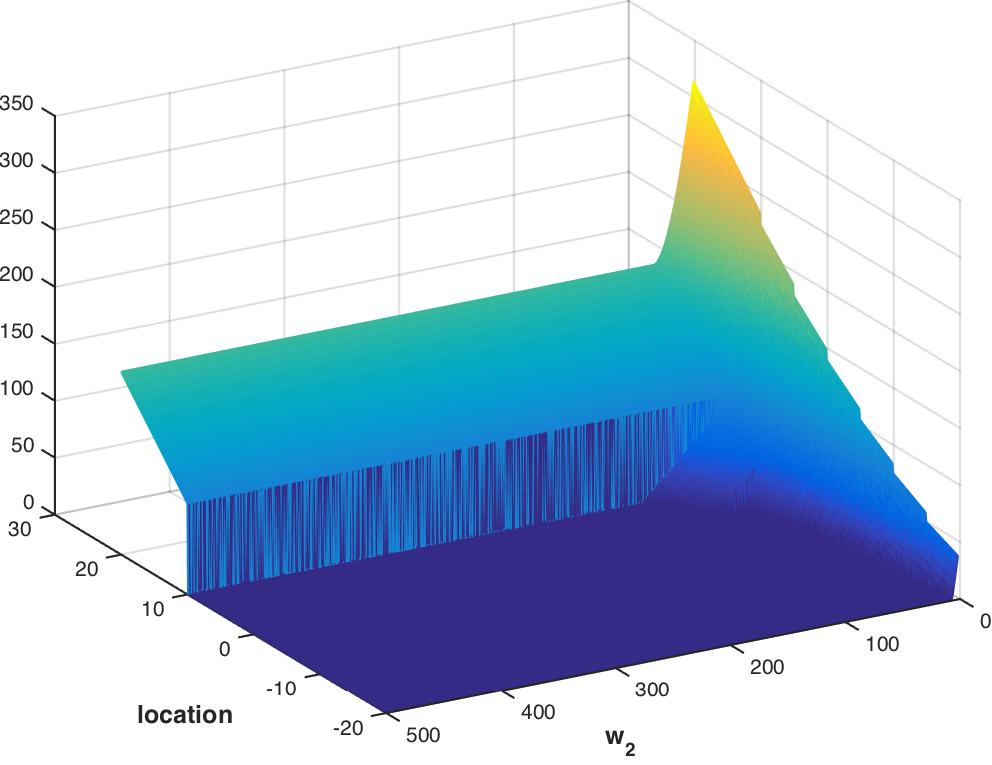
\includegraphics[width=0.8\linewidth, height=0.55\linewidth]{images/robot1d}
    \caption{The optimal value function for the multi-objective navigation domain. At low values of {\footnotesize $w_2$} the vehicle is willing to incur the movement cost to reach regions with higher linear reward.}
    \label{fig:vehicle1d}            
\end{figure}
%------------------------------------------------------------------------------

\subsection{Influenza Public Health Policy}
\label{sec:results_influenza}

Influenza viruses continuously challenge human hosts with new variants and cause complex epidemics. Compartmental models are widely used within epidemiology to investigate the spread of infection diseases such as Influenza. In this domain we investigate the efficacy of the public health policy of vaccination on a model of Influenza epidemiology by varying an infection rate parameter.

%The common components of both models can be defined as:
%\begin{itemize}
%    \item {\footnotesize $ \Action \in \left\lbrace 0, 0.25, 0.50, 1.0 \right\rbrace $} is the proportion to vaccinate 
%    \item {\footnotesize $ \Reward\left(\vec{w}, cost_{\mathtt{inf}}, cost_{\mathtt{vaccine}}, s, i, a \right) = w_1 \cdot \Reward_{\mathtt{inf}} + w_2 \cdot \Reward_{\mathtt{vaccine}}$} where, \\
%    {\footnotesize 
%        \abovedisplayskip=10pt
%        \belowdisplayskip=0pt
%        \renewcommand{\arraystretch}{1.5}
%        \begin{tabular}{ll}    
%            $ \Reward_{\mathtt{inf}}(i, cost_{\mathtt{inf}}) = $ &  $ $ \\
%            \qquad $ \begin{cases}
%            (i \geq 0) : & -cost_{\mathtt{inf}} \cdot i \\
%            \text{otherwise} : & 0 \\
%            \end{cases} $ & $ $ \\
%            $ \Reward_{\mathtt{vaccine}}(s, a, cost_{\mathtt{vaccine}}) = $ &  $ $ \\
%            \qquad $ \begin{cases}
%            (s \geq 0) : & -cost_{\mathtt{vaccine}} \cdot s \cdot a \\
%            \text{otherwise} : & 0 \\
%            \end{cases} $ & $ $ \\
%        \end{tabular}
%    } \\
%{\footnotesize $ cost_{\mathtt{inf}} $} is the incident cost of infection, akin to a burden of disease, and {\footnotesize $ cost_{\mathtt{vaccine}} $} is the unit cost of vaccination. \\    
%\end{itemize}

%\subsubsection{S-I Model}
%\label{sec:results_influenza_sd}
%
%A simple two compartment S-I epidemiological model is shown in Figure~\ref{fig:si_spec}.
%%------------------------------------------------------------------------------
%% Figure
%\begin{figure}[h!]
%    \centering
%    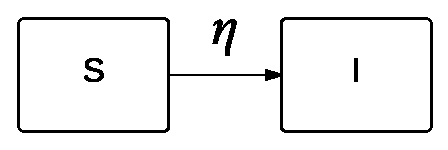
\includegraphics[width=0.3\linewidth, height=0.11\linewidth]{images/si}
%    \caption{An S-I model of Influenza epidemiology. {\footnotesize $ S $} and {\footnotesize $ I $} refer to the size of the susceptible and infected sub-populations, respectively. The infection rate is specified by {\footnotesize $ \eta$}. }
%    \label{fig:si_spec}            
%\end{figure}
%%------------------------------------------------------------------------------
%The S-I model can be formulated as a PHMDP as follows:
%\begin{itemize}
%    \item {\footnotesize $ \State = \left\langle s, i \right\rangle$}, where $ s $ and $ i $ are as defined above
%    \item The transition function {\footnotesize \Transition} for each state variable in {\footnotesize \State} is given by:    \\
%    {\footnotesize 
%        \abovedisplayskip=5pt
%        \belowdisplayskip=0pt
%        \renewcommand{\arraystretch}{1.5}
%        \begin{tabular}{ll}
%            $ \Transition\left( s' | s, i, a \right) =$ & $ \delta \left[ s' - (s - s \cdot (\eta + a)) \right] $ \\
%            $ \Transition\left( i' | s, i, a \right) =$ & $ \delta \left[ i' - (i + \eta \cdot s) \right] $ \\
%        \end{tabular}
%    }%
%    \item {\footnotesize $ \Action \in \left\lbrace 0, 0.25, 0.50, 1.0 \right\rbrace $} is the proportion of $ s $ to vaccinate 
%    \item {\footnotesize $ \Reward\left(\vec{w}, cost_{\mathtt{inf}}, cost_{\mathtt{vaccine}}, s, i, a \right) = w_1 \cdot \Reward_{\mathtt{inf}} + w_2 \cdot \Reward_{\mathtt{vaccine}}$} where, \\
%    {\footnotesize 
%        \abovedisplayskip=10pt
%        \belowdisplayskip=0pt
%        \renewcommand{\arraystretch}{1.5}
%        \begin{tabular}{ll}    
%            $ \Reward_{\mathtt{inf}}(i, cost_{\mathtt{inf}}) = $ &  $ $ \\
%            \qquad $ \begin{cases}
%            (i \geq 0) : & -cost_{\mathtt{inf}} \cdot i \\
%            \text{otherwise} : & 0 \\
%            \end{cases} $ & $ $ \\
%            $ \Reward_{\mathtt{vaccine}}(s, a, cost_{\mathtt{vaccine}}) = $ &  $ $ \\
%            \qquad $ \begin{cases}
%            (s \geq 0) : & -cost_{\mathtt{vaccine}} \cdot s \cdot a \\
%            \text{otherwise} : & 0 \\
%            \end{cases} $ & $ $ \\
%        \end{tabular}
%    } \\
%    {\footnotesize $ cost_{\mathtt{inf}} $} is the incident cost of infection, akin to a burden of disease, and {\footnotesize $ cost_{\mathtt{vaccine}} $} is the unit cost of vaccination.
%\end{itemize} 

%\subsubsection{S-I-R-S Model}
%\label{sec:results_influenza_sirs}

Influenza epidemiology is commonly investigated via a three compartment S-I-R-S model shown in Figure~\ref{fig:sirs_spec}.
%------------------------------------------------------------------------------
% Figure
\begin{figure}[h!]
    \centering
    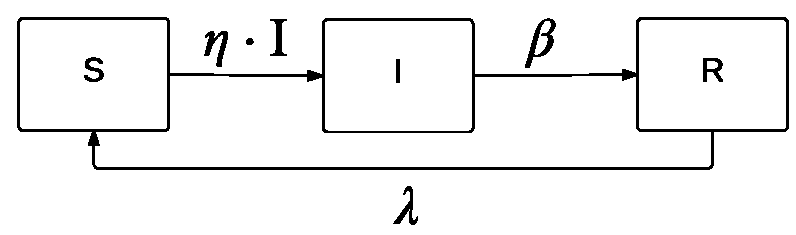
\includegraphics[width=0.5\linewidth, height=0.16\linewidth]{images/sirs}
    \caption{An S-I-R-S model of Influenza epidemiology.  {\footnotesize $ S $}, {\footnotesize $ I $} and {\footnotesize $ R $} refer to the size of the susceptible, infected and recovered sub-populations, respectively. The infection rate is specified by {\footnotesize $ \eta$}, {\footnotesize $\beta$} is the rate of recovery and {\footnotesize $\lambda$} is the rate of susceptibility.}
    \label{fig:sirs_spec}            
\end{figure}
%------------------------------------------------------------------------------

The domain is specified as follows:
\begin{itemize}
    \item {\footnotesize $ \State = \left\langle s, i, r \right\rangle$}, where $ s $, $ i $, and $ r $ are as defined above
    \item The transition function {\footnotesize \Transition} for each state variable in {\footnotesize \State} is given by:    \\
    {\footnotesize 
        \abovedisplayskip=5pt
        \belowdisplayskip=0pt
        \renewcommand{\arraystretch}{1.5}
        \begin{tabular}{ll}
            $ \Transition\left( s' | s, i, r, a \right) =$ & $ \delta \left[ s' - (s - \eta \cdot s \cdot i + \lambda \cdot r -a \cdot s) \right] $ \\
            $ \Transition\left( i' | s, i, r, a \right) =$ & $ \delta \left[ i' - (i + \eta \cdot s \cdot i - \beta \cdot i) \right] $ \\
            $ \Transition\left( r' | s, i, r, a \right) =$ & $ \delta \left[ r' - (r + \beta \cdot i - \lambda \cdot r) \right] $ \\            
        \end{tabular}
    }%
    \item {\footnotesize $ \Action \in \left\lbrace 0, 0.25, 0.50, 1.0 \right\rbrace $} is the proportion of $ s $ to vaccinate 
    \item {\footnotesize $ \Reward\left(\vec{w}, cost_{\mathtt{inf}}, cost_{\mathtt{vaccine}}, s, i, a \right) = w_1 \cdot \Reward_{\mathtt{inf}} + w_2 \cdot \Reward_{\mathtt{vaccine}}$} where, \\
    {\footnotesize 
        \abovedisplayskip=10pt
        \belowdisplayskip=0pt
        \renewcommand{\arraystretch}{1.5}
        \begin{tabular}{ll}    
            $ \Reward_{\mathtt{inf}}(i, cost_{\mathtt{inf}}) = $ &  $ $ \\
            \qquad $ \begin{cases}
            (i \geq 0) : & -cost_{\mathtt{inf}} \cdot i \\
            \text{otherwise} : & 0 \\
            \end{cases} $ & $ $ \\
            $ \Reward_{\mathtt{vaccine}}(s, a, cost_{\mathtt{vaccine}}) = $ &  $ $ \\
            \qquad $ \begin{cases}
            (s \geq 0) : & -cost_{\mathtt{vaccine}} \cdot s \cdot a \\
            \text{otherwise} : & 0 \\
            \end{cases} $ & $ $ \\
        \end{tabular}
    } \\
    {\footnotesize $ cost_{\mathtt{inf}} $} is the incident cost of infection, akin to a burden of disease, and {\footnotesize $ cost_{\mathtt{vaccine}} $} is the unit cost of vaccination.    
\end{itemize} 

%The {\footnotesize $\Action$} and {\footnotesize $\Reward$} components of the S-I-R-S model are as previously defined for the S-I model.

Figures~\ref{fig:influenza_sirs_value_function} and~\ref{fig:influenza_sirs_sensitivity} show the relationship between the susceptible sub-population {\footnotesize $s$} versus the infection rate {\footnotesize $\eta$} and the change in the infection rate {\footnotesize $\eta$} i.e. the sensitivity, respectively. The parameters of the model were set to {\footnotesize$ \beta = 0.27, \lambda = 0.23, cost_{\mathtt{inf}} = 95.0$} and {\footnotesize$cost_{\mathtt{vaccine}} = 33.0$}. In Figure~\ref{fig:influenza_sirs_value_function} we observe that the deleterious effect of low {\footnotesize $\eta$} are largely counteracted by the effect of {\footnotesize $ \lambda $}, the rate of susceptibility. For high values of {\footnotesize $s$}, a large {\footnotesize $\eta$} leads to a dramatic and rapid decline in value. Figure~\ref{fig:influenza_sirs_sensitivity} shows that the S-I-R-S model is highly sensitive to changes in the infection rate parameter {\footnotesize $\eta$}.
% and that small changes to {\footnotesize $\eta$} can lead to large changes in the parametric value function in Equation~\eqref{eq:vi_sdp_vfunc}.
%------------------------------------------------------------------------------
% Figure
\begin{figure}[h!]
    \centering
%    \begin{subfigure}[b]{0.5\textwidth}    
%        \centering
%        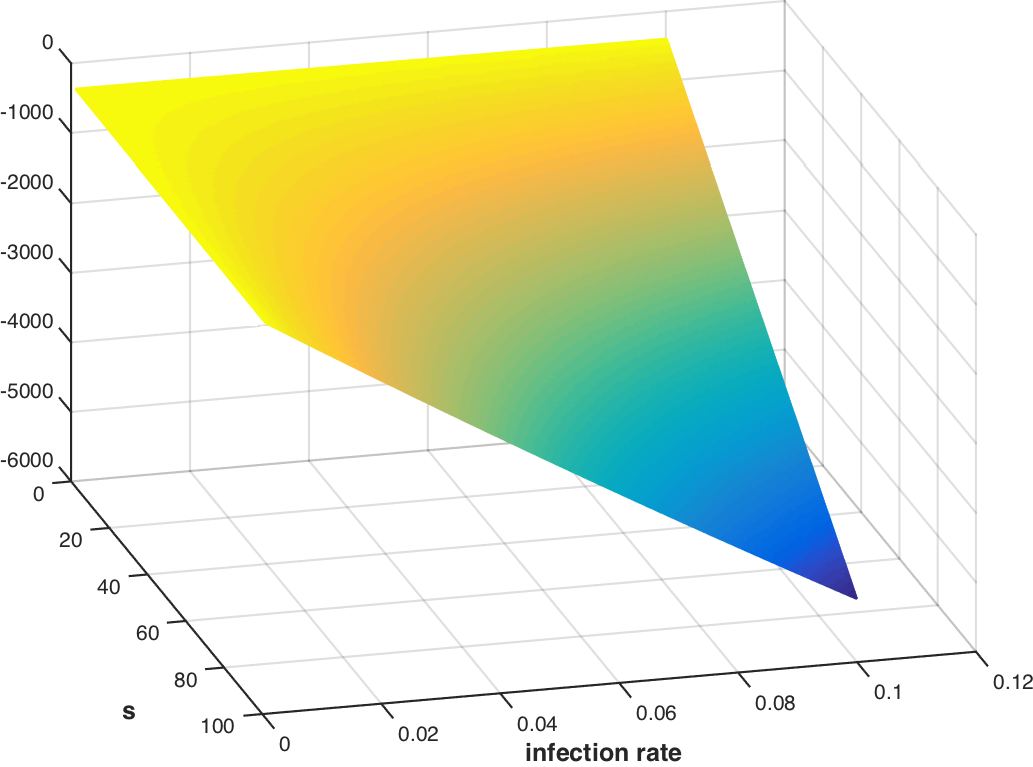
\includegraphics[width=0.8\linewidth, height=0.55\linewidth]{images/sd_infection_s}
%        \caption{S-I model.}
%        \label{fig:influenza_sd_value_function}
%        \vspace{1em}
%    \end{subfigure}  
    \begin{subfigure}[b]{0.5\textwidth}    
        \centering
        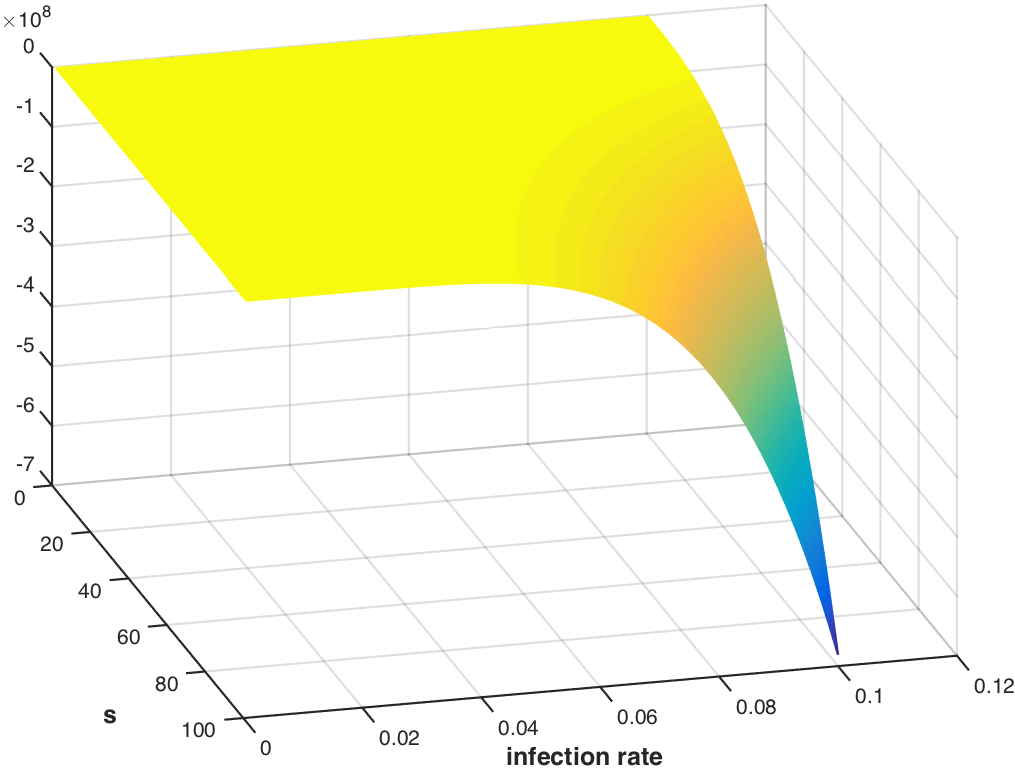
\includegraphics[width=0.8\linewidth, height=0.5\linewidth]{images/sir_infection_s}
        \caption{Susceptible vs. {\footnotesize $ \eta $}}
        \label{fig:influenza_sirs_value_function}
        \vspace{1em}
       \end{subfigure}         
    \begin{subfigure}[b]{0.5\textwidth}    
        \centering
        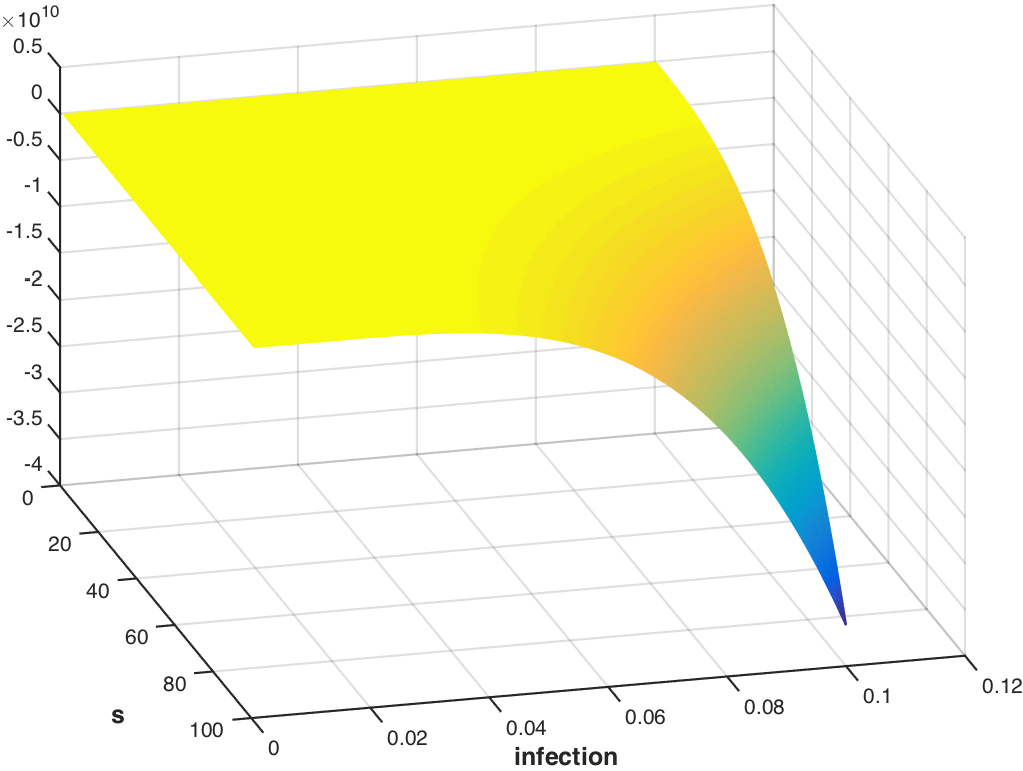
\includegraphics[width=0.8\linewidth, height=0.5\linewidth]{images/sir_infection_sensitivity}
        \caption{Susceptible vs. {\footnotesize $ \nabla \eta $} }
        \label{fig:influenza_sirs_sensitivity}
     \end{subfigure}         
    \caption{The effect of the infection rate {\footnotesize $\eta$} on the susceptible sub-population {\footnotesize $s$} under the S-I-R-S Influenza model. The S-I-R-S model is highly sensitive to higher values of {\footnotesize $\eta$}.}
    \label{fig:influenza_value_function}    
\end{figure}
%------------------------------------------------------------------------------

%------------------------------------------------------------------------------
%% Figure
%\begin{figure}[t!]
%    \centering
%    \begin{subfigure}[b]{0.5\textwidth}    
%        \centering
%        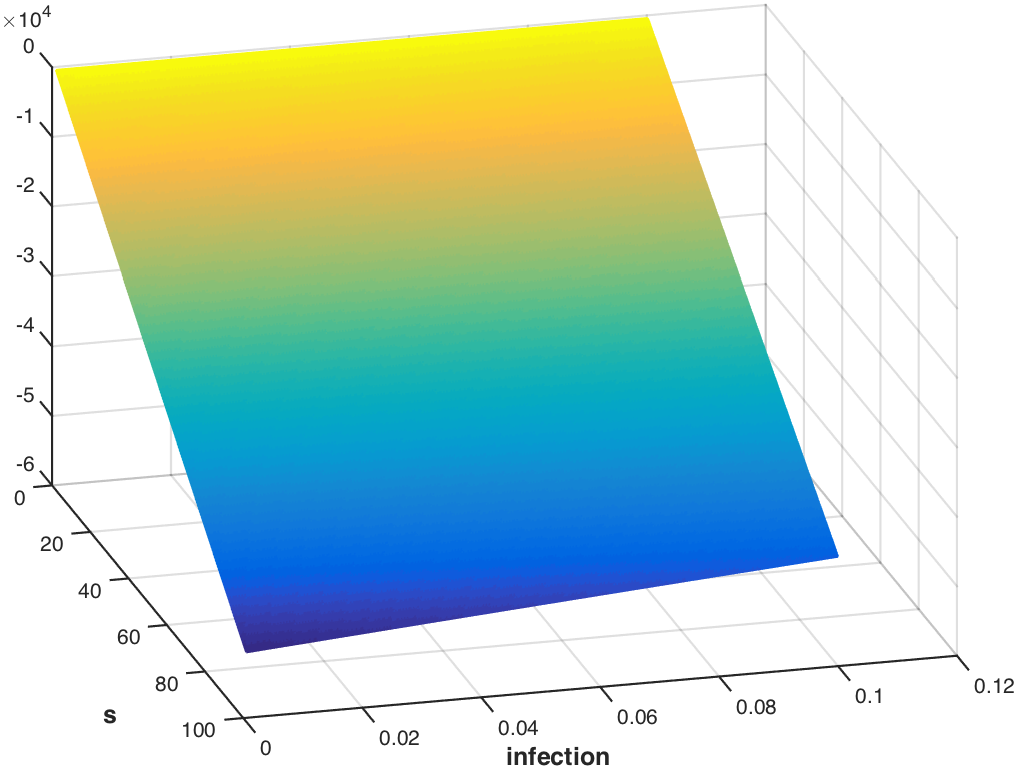
\includegraphics[width=0.8\linewidth, height=0.55\linewidth]{images/sd_infection_sensitivity}
%        \caption{S-I model.}
%        \label{fig:influenza_sd_sensitivity}
%    \end{subfigure}  
%    \begin{subfigure}[b]{0.5\textwidth}    
%        \centering
%        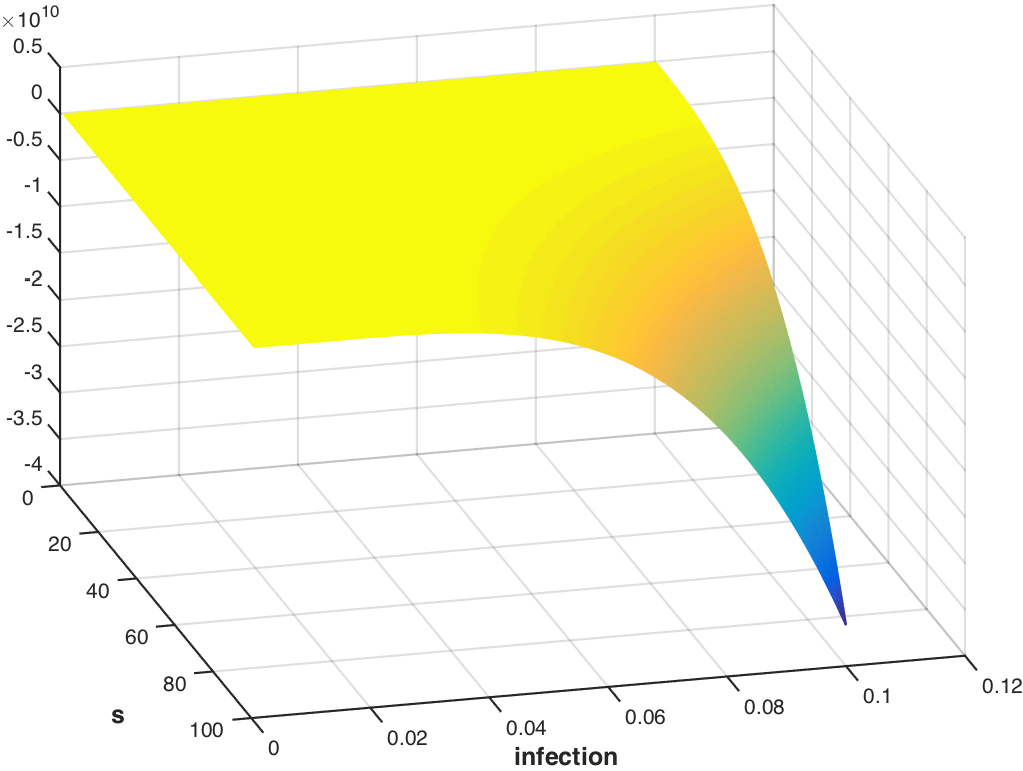
\includegraphics[width=0.8\linewidth, height=0.55\linewidth]{images/sir_infection_sensitivity}
%        \caption{S-I-R-S model.}
%        \label{fig:influenza_sirs_sensitivity}
%    \end{subfigure}  
%    \caption{The sensitivity of susceptible sub-population {\footnotesize $s$} to changes in the infection rate {\footnotesize $\eta$} under different Influenza model specifications. The S-I-R-S model is more sensitive to higher values of {\footnotesize $\eta$} than the S-I model. }
%    \label{fig:influenza_sensitivity}      
%\end{figure}
%------------------------------------------------------------------------------

\subsection{Optimal Execution}
\label{sec:results_oe}

Institutional investors often need to acquire or liquidate a number of shares within a given period of time. Indirect transaction costs are an important consideration for institutional investors who often want to transact a number of shares that exceeds the available liquidity i.e. there may not be a counterparty or counterparties that wish to take the other side of the trade at the same volume. There is a clear trade-off between the market impact of transacting immediately and the volatility of slow execution. 

In this domain we use a price impact model to investigate the optimisation of parameters within a static parameterized proportional liquidation policy, where the investor can vary the proportion of remaining inventory to sell. The domain is specified as follows:
\begin{itemize}
    \item {\footnotesize $ \State = \left\langle p, inv \right\rangle$}, where $ p $ is the price of the asset and $ inv $ is the inventory remaining
    \item {\footnotesize $ \Action \in \left\lbrace \pi\left( \theta \right) \right\rbrace$}, where {\footnotesize $ \theta \in \left( 0, 1\right)$} is the proportion of inventory to be sold
    \item The transition function {\footnotesize \Transition} for each state variable in {\footnotesize \State} is given by:    \\
    {\footnotesize 
        \abovedisplayskip=5pt
        \belowdisplayskip=0pt
        \renewcommand{\arraystretch}{1.5}
        \begin{tabular}{ll}
            $\Transition\left( p' | p, inv, \pi\left( \theta \right) \right) = $ & $\delta \left[ p' - (p + \kappa + \epsilon) \right] $ \\
            $\Transition\left( inv' | p, inv, \pi\left( \theta \right) \right) = $ & $\delta \left[ inv' - (inv - inv \cdot \pi\left( \theta \right)) \right] $ \\
        \end{tabular}
    }%
    {\footnotesize where $ \kappa $ and $ \epsilon$ are drift and discrete noise parameters, respectively.}
    \item {\footnotesize $ \Reward\left(p, p_0, inv, \pi\left( \theta \right) \right) = inv \cdot \left(\pi\left( \theta \right) \cdot p - p_0\right)$ }  
\end{itemize}

The investor aims to minimise \textit{price slippage}, which is defined as the difference between the theoretical benchmark price, {\footnotesize $p_0$}, and the actual price received.

Figure~\ref{fig:opt_execution} displays the optimal {\footnotesize$ \Horizon = 5 $} value function under the parameterized proportional liquidation policy. The parameters of the models were set to {\footnotesize$ \kappa = 1.65 \times 10^{-3}, p_0 = 10.0, p = 20.0$} and {\footnotesize $inv = \left\lbrace 0.0, 200.0\right\rbrace$}. It is clearly evident that the value function is maximised when the proportion sold, {\footnotesize $\pi\left( \theta \right) = 1.0$}, for all inventory settings. At this value of the parameter the investor maximises return by limiting exposure to price slippage.

%------------------------------------------------------------------------------
% Figure
\begin{figure}[h!]
    \centering
    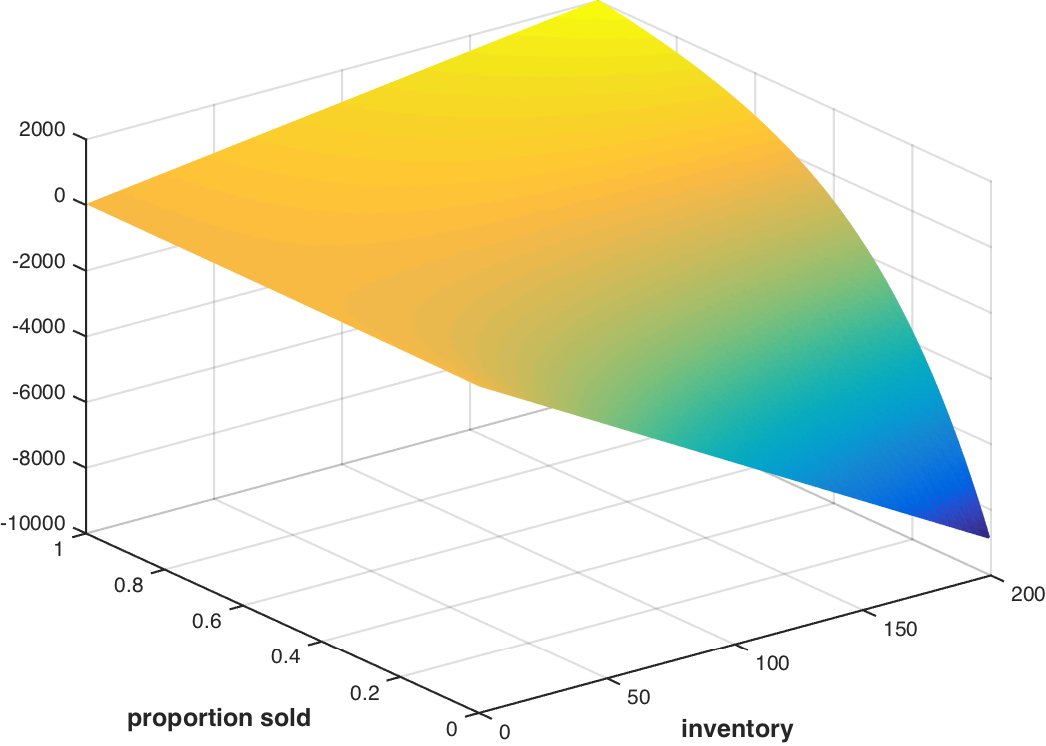
\includegraphics[width=0.8\linewidth, height=0.5\linewidth]{images/opt_execution_fraction}
    \caption{The optimal execution value function under the parameterized proportional liquidation policy. The reward obtained is maximised by increasing the policy parameter ({\footnotesize $\theta $}, the proportion sold) over all levels of inventory.}
    \label{fig:opt_execution}            
\end{figure}
%------------------------------------------------------------------------------